\section{Damara Benedikta}
\subsection {Apa itu fungsi library matplotib?}
Matplotip merupakan suatu library plotting 2D pada Phyton yang dapat menghasilkan sebuah gambar dengan bermacam-macam format. Matplotlib membantu mempermudah saat kita ingin membuat suatu plot, histogram, power spectra, grafik error,scatterplot,grafik batang dan sejenisnya hanya dengan menggunakan beberapa baris code. Sehingga sangatlah mempermudah kita dalam pembuatan diagram yang rapi dan cepat.
\subsection {Jelaskan langkah-langkah membuat sumbu x dan y di matplotlib}
Dimana vektor x dan vektor y harus memiliki ukuran yang sama. Vektor x adalah sumbu horizontal dan vektor y adalah sumbu vertical. 
\begin{enumerate}
	\item Pertama harus memastikan bahwa matplotlib.py plot sudah diimport kedalam file py
	\item Selanjutnya tentukan variable x dan y nya 
	\item Lalu tentukan berapa nilai variable x dan y nya 
	\item Kemudian variable tersebut akan dipanggil kedalam perintah plt.plot, seperti contoh plt.plot (x,y)
	\item Untuk dapat menampilkan hasil grafik tersebut gunakan perintah plt.show()
Berikut merupakan contoh codingan dan hasilnya : 

\lstinputlisting[firstline=9, lastline=15]{src/6/1174012/1174012.py}

\end{enumerate}
\subsection {Jelaskan bagaimana perbedaan fungsi dan cara pakai untuk berbagai jenis (bar,histogram,scatter,line) jenis plot di matplotlib}
\begin{itemize}
	\item Bar \newline
	Bar berfungsi untuk menampilkan suatu grafik bar dimana biasanya digunakan untuk menampilkan traffic 			penjualan 

\lstinputlisting[firstline=20, lastline=27]{src/6/1174012/1174012.py}

	\item Histogram \newline
	Histogram merupakan sebuah  grafik yang menampilkan frekuensi data menggunakan diagram batang, 			dimana angka-angka akan  dikelompokkan dalam rentang tertentu. Atau frekuensi pada  setiap elemen 			data yang ada di dalam daftar ditunjukkan menggunakan histogram. Angka yang 						dikelompokkan dalam bentuk rentang tertentu disebut dengan bins. 

\lstinputlisting[firstline=30, lastline=38]{src/6/1174012/1174012.py}

	\item Scatter \newline
	Scatter Diagram merupakan sebuah gambaran grafis yang terdiri dari sekumpulan titik-titikatau  (point) dari 		nilai sepasang variabel (Variabel X dan Variabel Y).

\lstinputlisting[firstline=41, lastline=55]{src/6/1174012/1174012.py}

	\item Line \newline
	Line merupakan sebuah plot yang sederhana dimana menggunkan diagram garis.

\lstinputlisting[firstline=9, lastline=15]{src/6/1174012/1174012.py}

	\item Pie \newline
	Pie merupakan sebuah diagram lingkaran dimana didalam lingkaran tersebut terdapat potongan yang 			membagi tiap tiap bagian.

\lstinputlisting[firstline=58, lastline=78]{src/6/1174012/1174012.py}

\end{itemize}
	
\subsection {Jelaskan bagaimana cara menggunkan legend dan label serta kaitannya serta kaitannya dengan fungsi tersebut}
legend berguna untuk menampilkan suatu keterangan tanda pada sebuah  grafik sedangkan label berguna untuk pemberian nama pada tanda tersebut. berikut merupakan syntax yang akan menampilkan legend dan label.

\lstinputlisting[firstline=41, lastline=55]{src/6/1174012/1174012.py}

\subsection {Jelaskan apa fungsi dari subplot di matplotlib, dan bagaimana cara kerja dari subplot, sertakan ilustrasi dan gambara sendiri dan apa parameternya}
Subplot adalah sebuah plot didalam dimana plot tersebut biasanya memiliki ukuran kecil sehingga dapat memuat plot 2 atau lebih plot dalam satu paket plot. 
Jika akan membuat 9 subplot maka yang harus dilakukan adalah membuat suatu perintah plt.subplot dengan parameter angka pertama 3 angka kedua 3 dan angka ketiga adalah 1 dimana angka pertama akan menjelaskan batas jumlah plot secara vertical, angka kedua akan menjelaskan batas plot secara horizontal, dan angka terakhir menjelaskan urutan plot tersebut.
iberikut merupakan contoh ilustrasi dari subplot:

\lstinputlisting[firstline=81, lastline=113]{src/6/1174012/1174012.py}

\subsection {sebutkan semua parameter color yang bisa digunakan}
\begin{enumerate}
	\item Parameter yang dapat digunakan adalah sebagai berikut CMYK
\end{enumerate}

\begin{itemize}
	\item C = Biru Muda
	\item M = Magenta atau Ungu
	\item Y = Kuning
	\item K = Hitam
\end{itemize}

\begin{enumerate}
	\item Parameter yang dapat digunakan selanjutnya adalah sebagai berikut RGB
\end{enumerate}

\begin{itemize}
	\item R = Merah
	\item G = Hijau
	\item B = Biru
\end{itemize}
\subsection {Jelaskan bagaimana cara kerja  dari fungsi hist, sertakan ilustrasi dan gambar sendiri}
Dalam Histogram sebuah  grafik yang menampilkan frekuensi data menggunakan diagram batang, dimana angka-angka akan  dikelompokkan dalam rentang tertentu.didalam histogram tidak mengacu pada sumbu x ataupun sumbu y.

\lstinputlisting[firstline=30, lastline=38]{src/6/1174012/1174012.py}

\begin{figure}[!htbp]
\centering
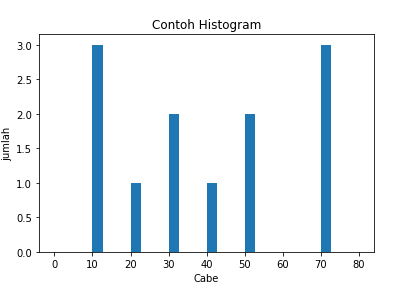
\includegraphics[scale=0.7]{figures/6/1174012/histo.PNG}
\caption{}
\label{}
\end{figure}

\subsection {Jelaskan lebih mendalam tentang parameter dari fungsi pie diantaraya labels,colors, startagle, shadow, explode,autopct}
\begin{itemize}
	\item Labels \newline
	Labels pada pie berguna untuk menambahkan keterangan pada pie dimana pada labels tersebut variabel 			didalamnya berisikan data array
	\item Colors \newline
	Colors pada pie berguna untuk mendefinisikan warna yang akan digunakan pada setiap grafiknya
	\item Startagle\newline
	Stargle pada pie berguna untuk mengatur perputaran potongan pada pie tersebut. dimana menggunakan 			satuan derajat pada setiap perputarannya.
	\item Shadow\newline
	Saddow pada pie berguna untuk pengaturan ketebalan bayangan pada sebuah pie.
	\item Explode\newline
	Explode pada pie berguna untuk pengaturan jarak pie yang akan dipotong keluar 
	\item Autopct\newline
	Autopct merupakan perhitungan dalam satuan persen dimana akan mengatur berapa digit angka yang akan 		muncul dibelakang 	koma.
\end{itemize}

\begin{figure}[!htbp]
\centering
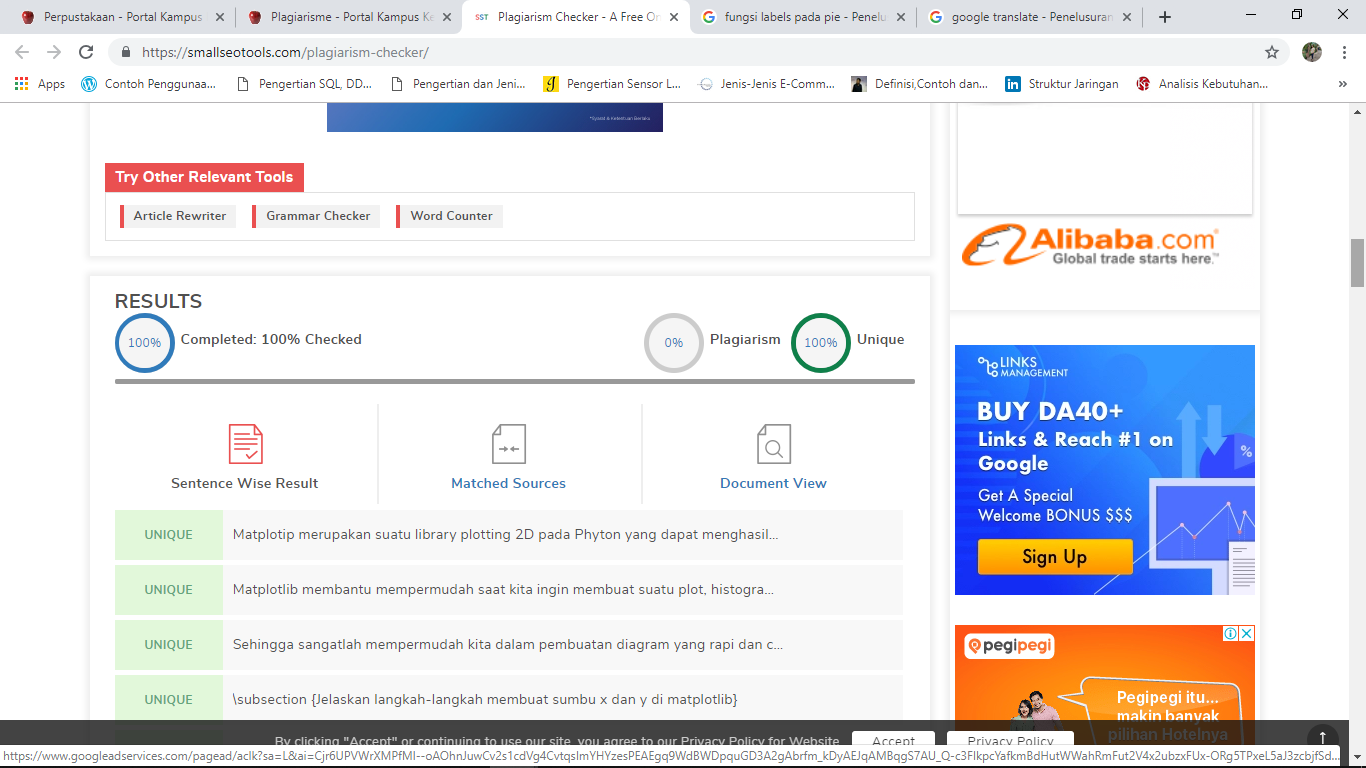
\includegraphics[scale=0.2]{figures/6/1174012/SSP.PNG}
\caption{plagiat}
\label{plagiat}
\end{figure}
